% !TEX root = ../lectures.tex
\section{Gamma-ray Absorption}

\begin{figure}[t]
\centering
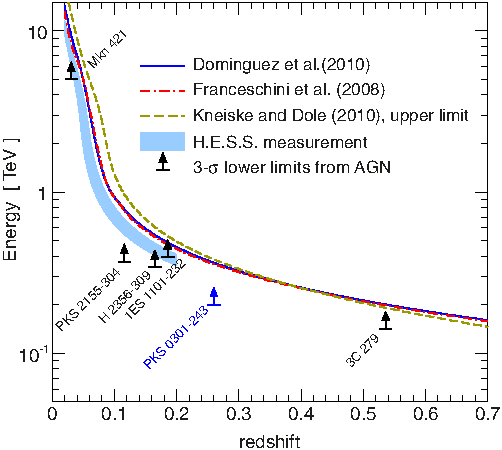
\includegraphics[width=0.5\textwidth]{figures/aa21639-13-fig6.pdf}
\caption{$\gamma$-ray horizon for differen EBL models. Some lower limits from AGN spectra measurements are shown~\cite{HESS2013aa}.}
\end{figure}

Extra-galactic gamma-rays undergo absorption during intergalactic propagation by interacting with photons in the diffuse radiation field, producing electron-positron pairs (\(\gamma + \gamma \rightarrow e^+ + e^-\)). This process depends on the energy threshold condition for opacity.

The square of the center-of-mass (COM) energy, \( s \), is a relativistic invariant:
%
\[
s = (P_a + P_b)^2 = m_a^2 + m_b^2 + 2(E_a E_b - \vb p_a \cdot \vb p_b) = m_a^2 + m_b^2 + 2E_a E_b (1 - \beta_a \beta_b \cos \theta)    
\]

For head-on collisions in the pair-production process \(\gamma + \gamma \rightarrow e^+ e^-\), the threshold energy in the LAB frame is:
%
\[
s = 2 E_\gamma \epsilon (1 + 1) = (2 m_e)^2 \rightarrow 4E_\gamma \epsilon = (2 m_e)^2 \rightarrow E_\gamma > \frac{m_e^2}{\epsilon}    
\]

For instance, a 1 TeV photon (\(E_\gamma = 10^{12}\) eV) interacts at the threshold with infrared photons (\(\epsilon \gtrsim 0.26\) eV).

The cross-section for pair-production, \(\sigma_{\gamma \gamma}(\beta^*)\), is given by:
%
\[
\sigma_{\gamma \gamma}(\beta^*) = \frac{3}{16} \sigma_{\rm T} (1-\beta^{*2}) \left[2 \beta^* (\beta^{*2}-2) + (3-\beta^{*4}) \ln \left( \frac{1+\beta^*}{1-\beta^*} \right) \right]
\]
%
where \(\beta^*\) is the velocity of the electron (or positron) in the CoM frame. 

The velocity \(\beta^*\) is determined by comparing the CoM energy with the energy in the CoM frame:
%
\[
2E_\gamma \epsilon(1- \cos\theta) = 4 E_e^{*2} \rightarrow \beta^* = \sqrt{1 - \frac{2 m_e^2 c^4}{E_\gamma \epsilon (1-\cos\theta)}}
\]
%
where I used
%
\[
E_e^* = \gamma^* m_e c^2 = \frac{1}{(1-\beta^{*2})^{1/2}} m_e c^2 = \sqrt{1 - \frac{2 m_e c^4}{x}}
\]

The cross-section reaches a maximum at \(x = 4 m_e c^4\), corresponding to \(\sigma(x) \simeq \sigma_{\rm T}/4\).

A 1 TeV photon most efficiently interacts with \(\sim 1\) eV photons. In the high-energy limit, the cross-section becomes inversely proportional to the energy product:
%
\[
\sigma_{\gamma\gamma}(\beta^*) \simeq \frac{3}{8} \frac{\sigma_{\rm T}}{\gamma^{*2}} \left[ \ln(4\gamma^{*2}) - 1\right] \propto \frac{1}{\gamma^{*2}} \simeq \frac{1}{E_\gamma \epsilon}
\]

That means that $\gamma$-rays can interact with all photons above the threshold but the cross-section decreases as $\epsilon$ increases (near threshold process).

The optical depth for \(\gamma\gamma\) absorption, \(\tau_{\gamma\gamma}(E_\gamma)\), takes into account all photons above the threshold:
%
\[
\tau_{\gamma\gamma}(E_\gamma) = \int_0^R \int_{4\pi} d\Omega (1-\cos\theta) \int_{\epsilon_{\rm th}}^\infty d\epsilon n_\gamma(\epsilon, \Omega, x) \sigma_{\gamma\gamma}(E_\gamma, \epsilon, \cos\theta)
\]

%%% PLOT WITH BACKGROUND FIELDS

%%% PLOT WITH SIGMA(X)

%%% PLOT WITH OPTICAL DEPTH

\subsection{Electromagnetic cascades}

TO BE DONE
